%%% 一个文档
% 导言：文件格式设置
\documentclass[UTF8]{ctexart}
% 该文档为中文文档，故用ctexart，英文文档则可用article
% 选项中的UTF8可有可无，因为这是默认编码
% \documentclass{article}

% 这些包里有一些数学公式
\usepackage[a4paper]{geometry}
\usepackage{amsmath}
\usepackage{commath}

% verbatim居中
\usepackage{fancyvrb}

% 图表
\usepackage{graphicx}
\usepackage{subfigure} % subfigure命令

% 这个包提供浮动体排版的方法
\usepackage{float}

% 这个包提供引用高亮与超链接
\usepackage{hyperref}

% 这个包可以打化学方程式
\usepackage{chemformula}

% 这个包可以打各种上标文字，但只能用于数学模式
\usepackage{accents}

% 这个包可以打各种上标文字
\usepackage{ruby}

\title{我的第一个 \LaTeX{} 文档}
\author{贺子旭}
\date{2023年5月30日}

% 正文
\begin{document}

% 生成标题
\maketitle

这是我的第一个 \LaTeX{} 文档。
它是一个由“pdfLaTeX”编译得到的文档，其文档类型为中文文章，即documentclass为ctexart。
我将用它来练习使用 \LaTeX ，方便未来学习写论文。
若有不熟悉的表达式可以在 cmd 输入查询“texdoc symbols”查找相关命令。

% 生成目录
\tableofcontents

\newpage

\section{简单公式}
	这是一个分数：$\frac{1}{2}$，
	它是由行内公式命令\$\textbackslash frac\{1\}\{2\}\$生成的；

	这是万有引力公式：
		\[F=G\frac{Mm}{r^2}\]

	这是一个显式公式，位于新的一行，但它没有编号，它是由
	\textbackslash[F=G\textbackslash frac\{Mm\}\{r\^2\}\textbackslash]
	生成的；

	这是用equation环境生成的勾股定理和余弦定理表达式：
	\begin{equation}
		a^2+b^2=c^2
	\end{equation}
	\begin{equation}
		a^2+b^2-2ab\cos{\theta}=c^2
	\end{equation}
	可以看到它右边有排列好的序号。其生成代码如下

	\begin{verbatim}
		\begin{equation}
			a^2+b^2=c^2
		\end{equation}
		\begin{equation}
			a^2+b^2-2ab\cos{\theta}=c^2
		\end{equation}
	\end{verbatim}

	顺便一提，上述代码是包裹一下环境 verbatim 里的

	同样，用equation*环境也能产生不排序的效果，如
	\begin{equation*}
		E = mc^2
	\end{equation*}

	这里是其他一些常见的公式：
	\begin{equation}
		\overline{x}=\frac{1}{n}\sum^{n}_{x=0}{x_{n}}
		\label{eq:average}
	\end{equation}
	\begin{equation}
		\sigma_{x}=\sqrt{\frac{1}{n}\sum^{n}_{x=0}{(x-\overline x)^2}}
		\label{eq:diff}
	\end{equation}
	其中，方程 ~\ref{eq:average} 为平均数公式，而方程 ~\ref{eq:diff} 为方差公式。

	只要在定义公式时使用 \textbackslash label\{eq:average\} 标记该公式，就可以通过 \textbackslash ref\{eq:average\} 引用该公式。

	这是一个化学方程式，它的生成方式是使用chemformula宏包的\textbackslash ch命令生成的，使用它时仍需要在equation环境内输入
	\begin{equation}
		\ch{CaCO3 + 2 HCl -> CaCl2 + H2O + CO2 ^}
	\end{equation}

\section{向量、矩阵与多行公式}
	物理学中常见的几个方程，它们是梯度、散度、旋度的计算公式；
	\begin{equation}
		\vec{\nabla}\phi
		=
		\left(
			\begin{array}{lcr}
				\frac{\partial \phi}{\partial x} \\
				\frac{\partial \phi}{\partial y} \\
				\frac{\partial \phi}{\partial z} \\
			\end{array}
		\right)
	\end{equation}
	% 下一个方程
	\begin{equation}
		\vec{\nabla}\cdot\vec{A} =
			\frac{\partial A_x}{\partial x}+
			\frac{\partial A_y}{\partial y}+
			\frac{\partial A_z}{\partial z}
	\end{equation}
	% 下一个方程
	\begin{equation}
		\vec{\nabla}\times\vec{A} =
		\left(
			\begin{array}{lcr}
				\hat{x} & \frac{\partial}{\partial x} & A_x \\
				\hat{y} & \frac{\partial}{\partial y} & A_y \\
				\hat{z} & \frac{\partial}{\partial z} & A_z \\
			\end{array}
		\right)
	\end{equation}

	这是一个方程组，在equation环境中用“\textbackslash left \textbackslash \{”与“\textbackslash right.”包裹起来，
	并用 marix 环境对齐。
	\begin{equation}
		\left\{
			\begin{matrix}
				x+y+z=0  \\
				x+2y+z=1 \\
				x+y+2z=2 \\
			\end{matrix}
		\right.
	\end{equation}

	这是一个偏微分方程组，对齐用的是 aligned 环境。
	\begin{equation}
		\left\{
			\begin{aligned}
				\frac{\partial}{\partial t} \rho           & + \vec{\nabla} \cdot (\rho \vec{u})                       & = 0  \\
				\frac{\partial}{\partial t} (\rho\vec{u})  & + \vec{\nabla} \cdot (\rho \vec{u}\vec{u}+p\vec{\vec{I}}) & = 0 \\
				\frac{\partial}{\partial t} (\rho\epsilon) & + \vec{\nabla} \cdot (\vec{u}(\rho\epsilon+p))            & = 0 \\
			\end{aligned}
		\right.
	\end{equation}

\section{文件导入}
	这是待导入文件，其中包含一个公式
\begin{equation}
	\left(
		\begin{matrix}
			x^{'(0)} \\
			x^{'(1)} \\
			x^{'(2)} \\
			x^{'(3)} \\
		\end{matrix}
	\right)
	=
	\left(
		\begin{matrix}
			\gamma      & \gamma\beta & 0 & 0 \\
			\gamma\beta & \gamma      & 0 & 0 \\
			0           & 0           & 1 & 0 \\
			0           & 0           & 0 & 1 \\
		\end{matrix}
	\right)
	\left(
		\begin{matrix}
			x^{(0)} \\
			x^{(1)} \\
			x^{(2)} \\
			x^{(3)} \\
		\end{matrix}
	\right)
\end{equation}
	这是另一个输入文件，其内容为：hello。

	\textbackslash input 功能类似于C语言的 \#include 功能，相当于将文档拼接起来。
	单独部分的文件多半不能通过编译。

\section{字体与字号}
	衬线字体笔画直，存在笔锋装饰，例如：宋体、Times New Roman
	
	无衬线字体（\textbackslash textsf\{我需要的Words\}）案例：
	
	\textsf{黑体，black}
	

	有衬线字体（\textbackslash textrm\{我需要的Words\}）案例：
	
	\textrm{黑体，black}

	word黑体坑：“simhei”非商用字体，需要使用的是“黑体”。


	意大利斜体（\textbackslash textit\{我需要的Words\}）案例：
	
	\textit{意大利斜体、italic}

	意大利斜体主要用于强调，可以用“\textbackslash emph”命令替换，
	如：
	
	这是一个\emph{需要强调的}的文本。
	This is an text \emph{need to be emphasised}.

\newpage

\section{图片与表格}
	\begin{figure}
		\centering
		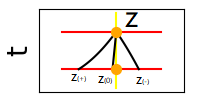
\includegraphics[width = 0.4 \textwidth]{../pictures/Charateristic Line.png}
		\caption{这是一张插图，这张插图是过一个点的特征线}
		\label{fig:chrp}
	\end{figure}
	插图 ~\ref{fig:chrp} 描述的是一组特征线。这张图片没有采用[h]或[t]标注，自动浮动到页首。
	
	插图 ~\ref{fig:sign} 使用[h]标定，则出现在其被引用位置
	\begin{figure}[h]
		\centering
		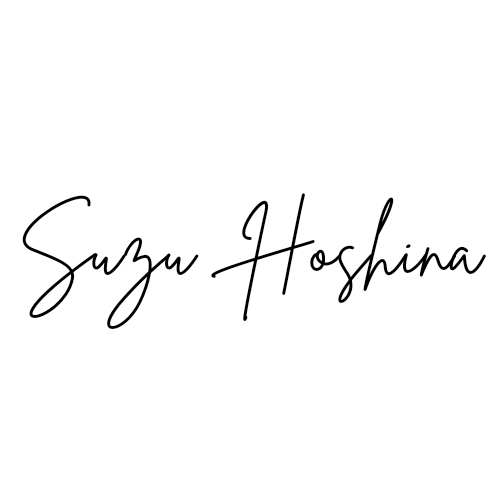
\includegraphics[width = 0.3\textwidth]{../pictures/Signature.png}
		\caption{这是一张插图，这张插图是铃宝的签名}
		\label{fig:sign}
	\end{figure}

	其他标记如以下表格所示
	\begin{table}[H]
		\begin{center}
			\begin{tabular}{c|c}
				\hline
				标签		&	含义 \\
				\hline
				[t]		&	置顶 \\ \relax
				[b]		&	置底 \\ \relax
				[p]		&	换页 \\ \relax
				[h]		&	视情况插入中段 \\ \relax
				[H]		&	强制插入中段 \\ 
				\hline
			\end{tabular}
		\end{center}
		\caption{图表位置调整标签}
		\label{table:location}
	\end{table}
	该表格使用\textbackslash table 环境与\textbackslash tabular 环境实现。
	\textbackslash tabular 需要用{}

\section{参考文献引用}
	这是一个引用参考文献的样例。 \cite{texbook}

\section{自定义命令与自定义环境}
	利用\textbackslash newcommand命令可以定义自己需要的命令。
	自己定义的命令与内置命令一样，需要以\textbackslash 开头。
	而定义的参数则用井号开头。其基本格式如下

	\begin{center}
		\begin{BVerbatim}
\newcommand{命令}{命令含义}
\newcommand{命令}[参数个数]{命令 #参数编号 的含义}
		\end{BVerbatim}
	\end{center}

	例如：
	\begin{center}
		\begin{BVerbatim}
\newcommand{\density}{\rho}
\newcommand{\red}[1]{\textcolor{red}{#1}}
\newcommand{\myint}[3]{\displaystyle\int_{1}^{#2} #3}
		\end{BVerbatim}
	\end{center}

	\newcommand{\density}{\rho}
	\newcommand{\red}[1]{\textcolor{red}{#1}}
	\newcommand{\myint}[3]{\displaystyle\int_{#1}^{#2} #3}
	使用这两条命令的文本样例：

	\begin{center}
		\red{密度定义式}：$\density(\vec{r}) = \frac{dm}{dV}$

		\red{牛顿-莱布尼茨公式}：$F(b)-F(a)=\myint{a}{b}{f(x)dx}$
	\end{center}

	环境的定义用的是\textbackslash newenvironment 命令实现。其基本结构如下
	\begin{center}
		\begin{BVerbatim}
\newenvironment{环境名称}[参数个数]{文前命令}{文后命令}
		\end{BVerbatim}
	\end{center}
	
	其中，在文前命令将在\textbackslash begin{环境}阶段处理，
	而文后命令将在遇到 \textbackslash end{环境} 阶段处理。

	例如：

	\begin{center}
		\begin{BVerbatim}
\newenvironment{note}{
	\par \vspace{0.5cm}
	\hrule
	\vspace{0.1cm}
	\par \small
}
{
	\par \vspace{0.1cm}
	\hrule
	\par\vspace{0.5cm}
	\normalsize
}
		\end{BVerbatim}
	\end{center}

	使用该命令
\newenvironment{note}{
	\par \vspace{0.5cm}
	\hrule
	\vspace{0.1cm}
	\par \small
}
{
	\par \vspace{0.1cm}
	\hrule
	\par\vspace{0.5cm}
	\normalsize
}
	\begin{note}
		这是一条笔记

		这个环境是我用\textbackslash newenvironment自创的
	\end{note}

	更加精细的命令与环境定义可以参考\red{xparse}宏包。

\section{其他}
	enumerate环境可以创造小编号枚举，而 itemize 环境则对应加点不编号的环境。
	后者常见于PPT写作。

	minipage环境常用于分页。

	举例：
	\par \vspace{0.5cm}
	\begin{minipage}[h]{0.48\textwidth}
		常见的光学表面清洗方法有
		\begin{enumerate}
			\item 擦拭法
			\item 化学清洗法
			\item 超声清洗法
			\item 激光清洗法
			\item 等离子体清洗法
		\end{enumerate}
	\end{minipage}
	\hspace{2mm}
	\begin{minipage}[h]{0.48\textwidth}
		二氧化碳雪清洗方法优势
		\begin{itemize}
			\item 成本低
			\item 无污染
			\item 面型破坏小
			\item 无需二次处理
			\item 无需拆卸仪器
		\end{itemize}
	\end{minipage}

	\vspace{1cm}
	\textbackslash subfigure是figure环境下的命令，其依赖 subfigure 包，用于创建并列排放的图片。
	
	使用方法
	\begin{verbatim}
		\subfigure[小图标签]{\includegraphics[width=宽度]{图片路径}}
	\end{verbatim}

	用例：
	\begin{figure}[H]
		\centering
		\subfigure[特征线]{\label{fig:chrp2}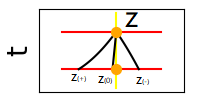
\includegraphics[width=0.4\textwidth]{../pictures/Charateristic Line.png}}
		\subfigure[签名]{\label{fig:sign2}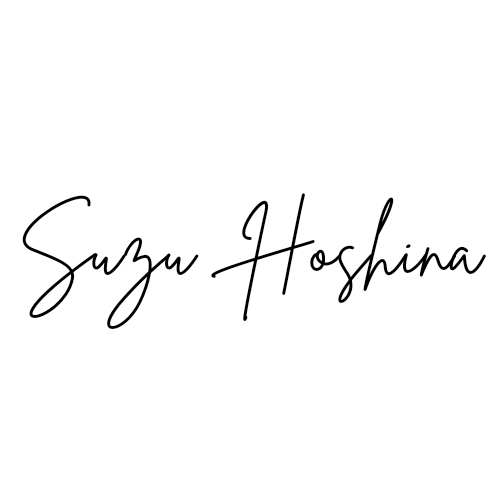
\includegraphics[width=0.4\textwidth]{../pictures/Signature.png}}
		\label{fig:subfig}
		\caption{子图案例}
	\end{figure}
	图 \ref{fig:subfig} 展示了子图的使用，其中图 \ref{fig:chrp2} 和图 \ref{fig:sign2} 为其对应两个子图。

	同样，subfig的subfloat也有同样的功能与使用方法。

	equation下的split环境适用于连等号环境。例如
	\begin{equation}
		\begin{split}
			(3 + 5) \times 6 + 7 \times 6 - 6 \div 3 &= 8 \times 6 + 7 \times 6 - 6 \div 3 \\
			&= 48 + 7 \times 6 - 6 \div 3 \\
			&= 48 + 42 - 6 \div 3 \\
			&= 48 + 42 - 2 \\
			&= 90 -2 \\
			&= 88
		\end{split}
	\end{equation}

	gather环境不需要equation环境进行包裹直接使用，该环境可以合并多个并排的公式
	例如：
	\begin{gather}
		m_{v} = m_0\frac{1}{\sqrt{1-\left(\frac{v}{c}\right)^2}}   \label{eq:SR1} \\
		\vec{p}_v = m_v\vec{v}                                     \label{eq:SR2} \\
		E = mc^{2}                                                 \label{eq:SR3} \\
		E^{2} = \left(mc^{2}\right)^{2} + (pc)^2                   \label{eq:SR4}
	\end{gather}
	方程 ~\ref{eq:SR1}、方程 ~\ref{eq:SR2}、方程 ~\ref{eq:SR3}、方程 ~\ref{eq:SR4} 是狭义相对论中几个重要的结论。
	
	\verb|\verb|命令是行内的\verb|verbatim|环境，其语法如下

	\begin{center}
		\begin{BVerbatim}
\verb|需要包含的文字|
		\end{BVerbatim}
	\end{center}

	利用\verb|\verb|命令可以很容易地书写~\LaTeX~命令，如：\verb|\section{章节}|、\verb|$a^2+b^2=c^2$|、\verb|\emph{需要强调的文字}|等等。

	利用\verb|accents|包内的\verb|accentset|命令可以完成上标文字的书写。如~$\accentset{\cdot}{x}$、
	$\accentset{\rightarrow}{u}$、$\accentset{some words}{some other words}$~\dots
	该上标功能只能在数学功能内使用，而要给文字注音则需要使用\verb|ruby|宏包的内容，如
	

	
\bibliographystyle{plain}
\bibliography{../citations/References}


\end{document}
